\documentclass[../eva1_scion.tex]{subfiles}
\begin{document}
    \chapter{Results}
    In this chapter we describe the current state of the proposed SCION architecture. We examine the anatomy of \textit{Isolation Domains} (ISD) and elaborate how the SCION control and data plane work.

    \section{Isolation Domains}
    SCION is designed for easy adoption by current BGP ASes, therefore it adopts and alters some ideas from BGP like the idea of an Autonomous System (AS) which, like in BGP, repesents the smalest organisational unit. However, SCION introduces an additonal organisational unit called the Isolation Domain (ISD). The structure of an indivual ISD is ilustrated in \ref{fig:isd}a. 

    An ISD shares a common set of operational rules and share a set of trust roots. It is expected that ISDs will grow along social, political and econmical borders and structures \cite{scion_2011}. Giving these technical implemtations a common legal and contractual framework and social context, from which enforcability and a meaningful (for humans) sense of trust can be derived. To emulate these realworld structures, SCION supports recursive ISDs  which inherint trust roots and rules from their parent ISDs \cite{scion_2011}. As an example one might imagine the tier-1 providers in a country forming the ISD core of a country level ISD, which is member of an ISD representing larger geopolitical entity like the EU. Inside a country there might be a group of ASes which have stronger requirements regarding security and trust than the rest the ISD, thus they may form a subISD inside the subISD of the country. One such example may be military and its associated organisations.


    \subsection{IDS Structure}
    As shown in ilustration \ref{fig:isd}a the main structure of an IDS is an undirected graph formed by a set of core ASes in the ISD core, client ASes and biderectional links between individual ASes. ASes may be connected by multiple redundant links. Although a link always carries biderctional traffic, there is an implied top down hirarchy of providers and consumers between the tiers in the graph. As in BGP a pair of ASes may enter an peering agreement, which is ilustrated is a dashed line. Links are also called path segments.

    An ISD core is comprised of multiple core ASes which form fully connected clique and a logical. The ISD core hosts numerous function such as the ISDs certificate authority, core beacon-, certificate-, path-, and address-servers.The ISD core also maintains the \textit{Trust Root Configuration} TRC. The ISD core also provides links to other ISDs. The requirement to become a core AS is usually sufficient size or importance to offer direct connections to other core ASes in other ISDs, as well as the ability to repicate the other core services listed above \cite{scion_2011}.

    An unassociated AS can join an existing ISD by purchasing connectivety from an ISD which is allready member of a given ISD. This requires the joining AS to accept the TRC and operational rules of the ISD it whishes to join. Each AS can be member of multiple ISDs.

    \begin{figure}[ht]
        \centering
        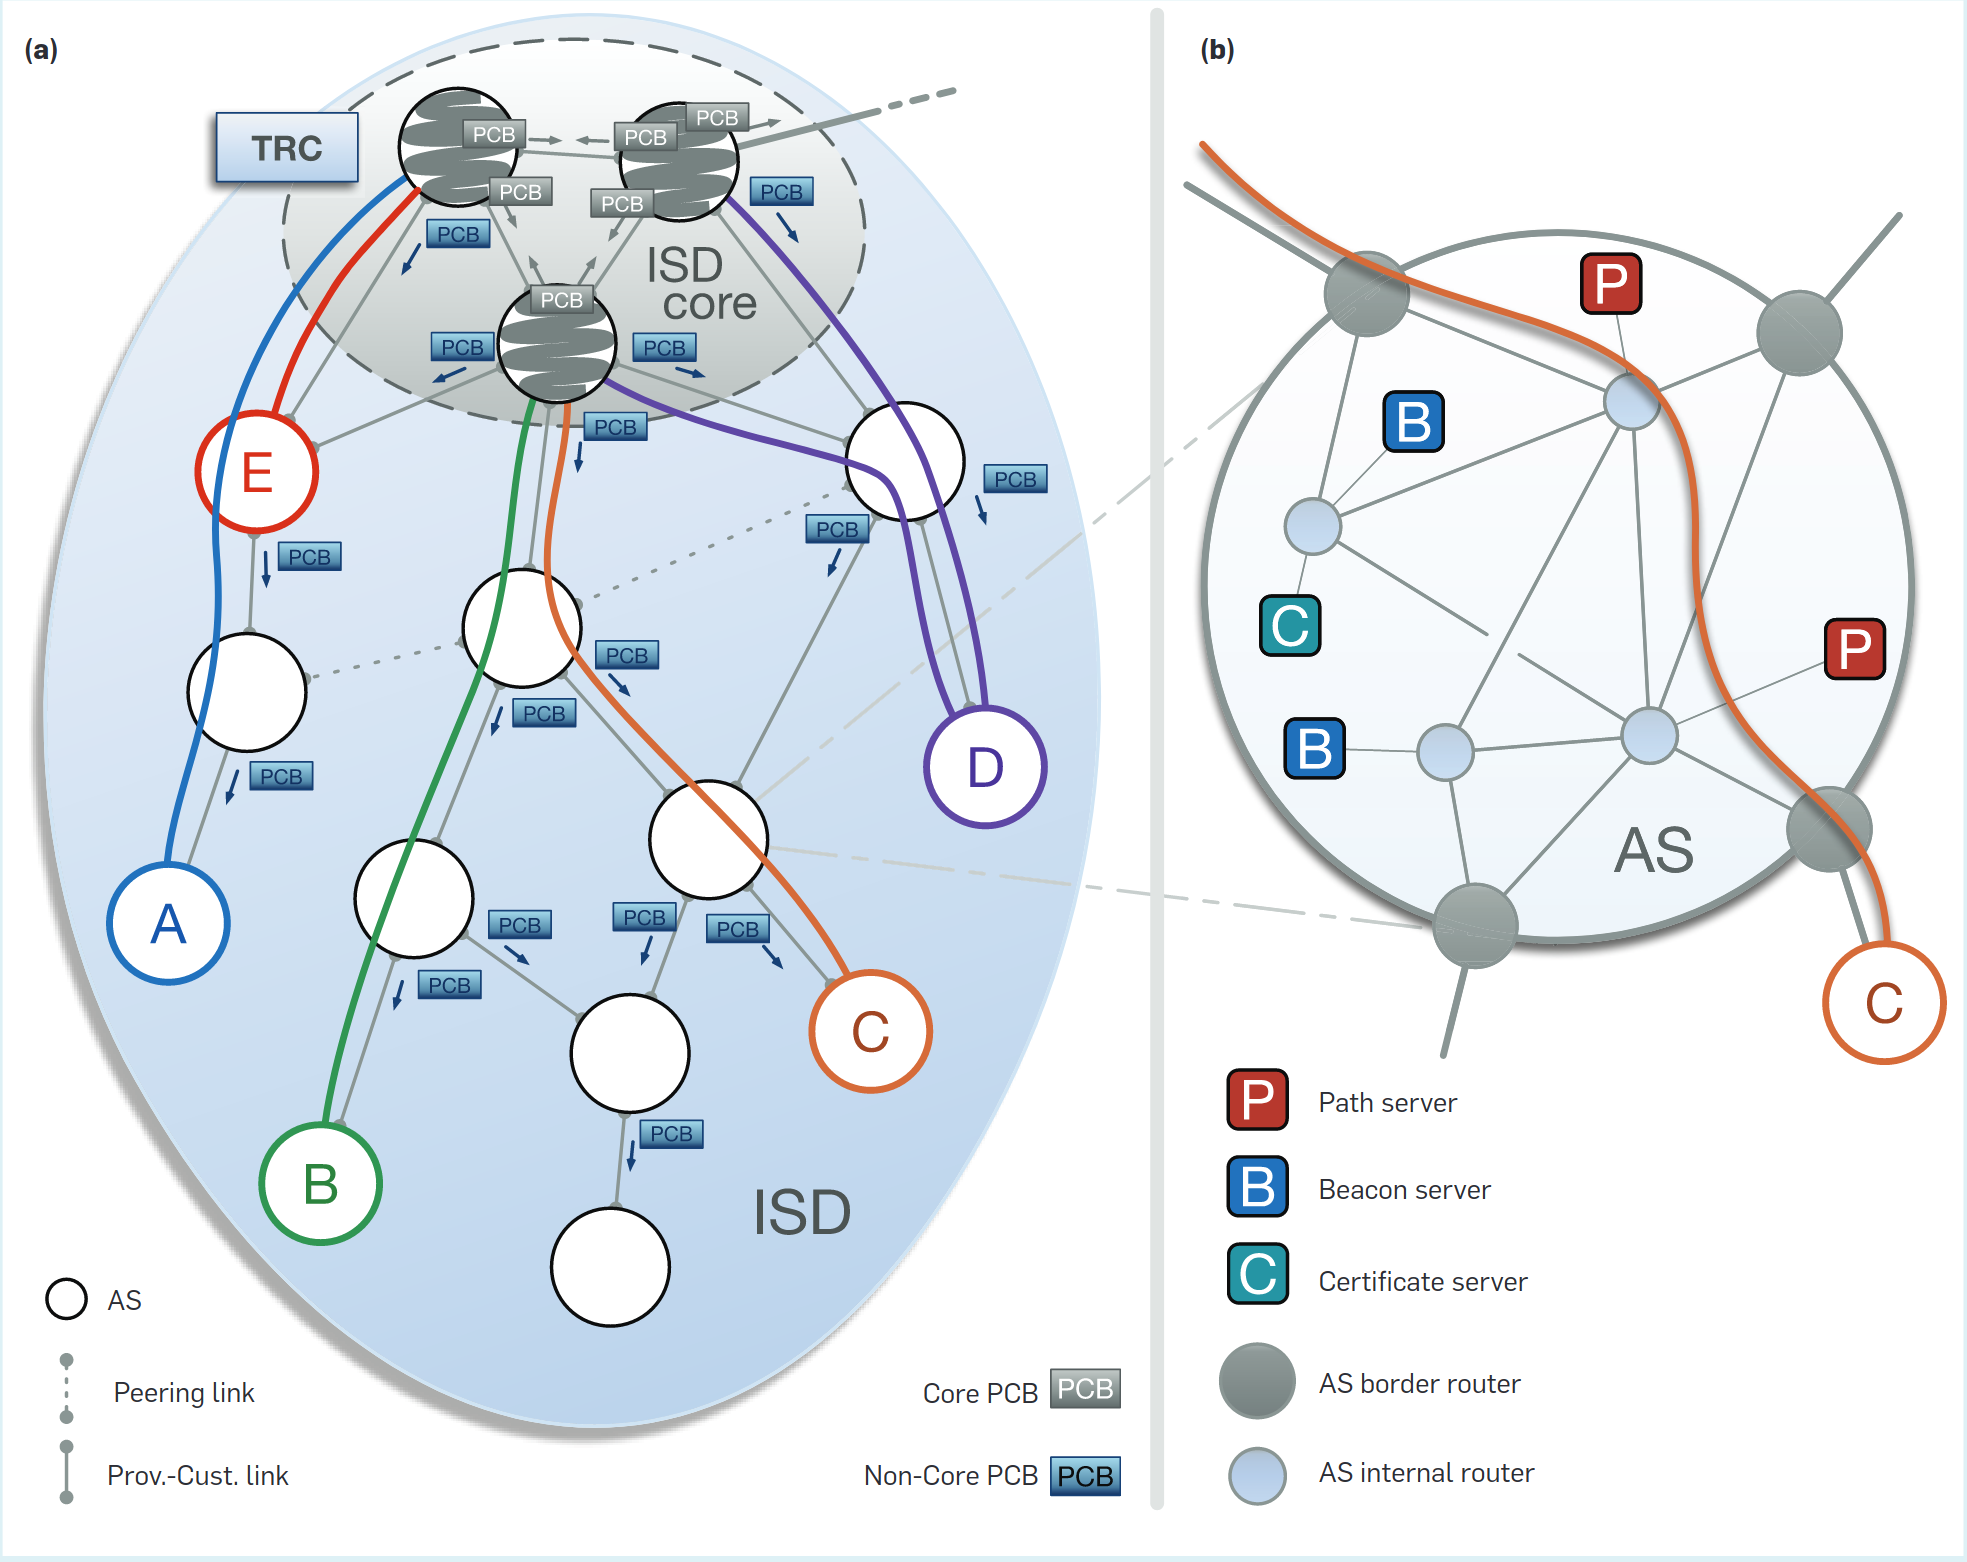
\includegraphics[width=0.8\linewidth]{scion_isd.png}
        \caption{Internal structure of an ISD. From \cite{scion_2017}}%
        \label{fig:isd}
    \end{figure}

    \subsection{AS and ISD Componants}

    In the following we will explore the componantes which are required to run an SCION AS and by extension a ISD since an ISD usually replacates all or most core services for caching reasons.

    SCION ASes look similar too their BGP cousins so fare as that they have internal routers and border routers and a set of routes through the AS. These ensure connectivity inside the AS and to neighbouring ASes. Border routers must be SCION capable and must addhere to the common rules agreed upon inside the ISD, however each AS is free to choos its internal structure. Such as the intra domain routing protocol and adressing schema. Initially SCION was designed to employ \textit{Accountable IP} (AIP) \cite{scion_2011, aip_2008} in all ASes, however this requirement was relaxed later in favour of interoperability and ease of adoption \cite{scion_2017}. Because of the way SCION fowards packets, there is also no need for a uniform addressing schema between ASes (see \ref{sec:data_plane}).

    In addition each AS needs at least a beacon server, a certificate server and a path server. Beacon servers are responbsible for path discovery and are required for beaconing process described in section \ref{ssec:beaconing}. Path server are repsonsible for caching and disimination of path information. They are involved in path resolution and assembly discussed in section \ref{ssec:path_assembly}. As SCION makes extensive us of certificates to validate paths and entities \cite{scion_2011}, certificate servers are deployed to cache and provide certificates in an AS.

    A core AS differs from other ASes in serveral important aspects. Most importantly core ASes have border routers which are connected to cores ASes in neighbouring ISDs. Further, the beacon servers in the core ASes also take part in inter ISD beaconing (see section \ref{ssec:beaconing}), thus their path servers also hold path information on how to reach neighbouring ISDs. As mentioned above the ISD core is responsible for maintaining the trust root configuration (TRC).

    The \textit{Trust Root Configuratio} (TRC) is policy which governs the operations of an ISD. The TRC lists the trust roots used in an ISD and thus is the central anchor of trust in an ISD. It is negotiated between the members of the ISD core and all ASes whishing to join an ISD need to accept the TRC. Neighbouring ISDs acknowledge an ISDs TRC by signing it. This makes ASes communicting across ISD bordes able to trust signatures originating from an neighouring ISD. Each TRC also holds a number of policies on how the TRC is used and. Modifications to the TRC are only possible of multiple core ASes signe updated TRC, which prevents a rouge core AS from corupting the TRC. The number of required signatures for different kinds of changes is governed by the policies encoded in the TRC.

    \section{Control Plane}
    Until now we looked at the static componants which make up an ISD, however the real world internet is not a static thing, so an ISD isn't either. To better manage complexity SCION is devided into a controll plane and a data plane. The control plane is concerned with discovering and maintaining paths, while the data plane uses these paths in the processes of path assembly and packet fowarding. This division not only isolates complexity, but also isolates failures. As long as there are paths available to forward packets on, the data plane can operate without disruption, even if parts of the control plane are disrupted.

    \subsection{Path Discovery by Beaconing}\label{ssec:beaconing}
    As mentioned above SCION has taken inspiration form BGP, the paths discovery mechanism is an other place where this is evident. Like in BGP, SCION uses a beaconing process to discover all available paths between ASes. However unlike in BGP in SCION beacons are not broadcast by every AS to every connected AS, also each AS has control over the paths by which paths it would like to by reachable. In BGP an AS has no control over which routes its neighbouring ASes propagate. Beacons in SCION are called \textit{Path-Segment Construction Beacon}s (PCB) and are  sent from beacon servers in the ISD core to travle down the ISD graph as an policy constrained multipath flood. \cite{scion_2011}.

    Initialy the path server in a core ISD issues a PCB containing only the exit interface it originates from and the current version number of the TRC. A path server in a neighbouring AS receiving an incomming CP will first check the validity of the beacon by checking its signature. Then it goes on to process the PCB. First of all the version number of the TRC is checked and if necessary fetch the new TRC from the AS it received the PCB from. After adding its own path information to the PCB, the beacon server forwards the PCB to all its client ASes \ref{scion_2011}.

    Before forwarding the PCB the path server creates a record of the ingress inteface, egress interface, and available peers and then appends it to the PCB. These fields are called \textit{Opaque Fields} and are each protected by a MAC. Important to note is that only there is no requirement for other ASes to be able to interpret this field, because during packet fowarding an AS only has to read only the fields it has created itself (see section \ref{ssec:pcfs}). Thus this field is \textit{opaque} to other ASes. The new PCB, together with the old PCB information, is cryptographically signed before it is sent out, which leads to an onion like structure of signatures, protecting each step in the forwarding chaine from tampering \cite{scion_2011}. In this way a PCB accumulates verifyable path information as a so called path-segment while it is forwarded through the ISD. The information received in PCBs is cached in the local path servers, so endhosts in an ISD have a way to look up path information. Important to note is that PCBs are not sent out through peering links as this would lead douplicate paths or might lead to intra-ISD beacons leaking into other ISDs.

    PCBs traveling down collect what are called down paths, but since all paths forward packets bidirectionally, each down-segment can be converted into an up-segment by inverting the order or traversed ASes. This one way propagation of PCBs has an important consequence: An AS always knows an up-path back to the ISD core, but it does not know how the reach other AS or ISDs, thus down-paths to other ASes must always be queried from the paths servers in the ISD core. Once an AS has received a number of path-segments it can register some of them as down-paths segmemts with the core path servers in the ISD core. This gives an AS control over which down-paths are made available to other ASes and creates unique ability to control by which paths it whishes to be reached.

    When selecting down-paths an AS tries to select as diverse paths as possible in order reach maximum redudancy. This makes SCION an ineherently multipathed system. Apart from path diversity, ASes can select for many different quality measure in their paths like low latency or anonymous forwarding capability along the whole path \cite{scion_2011}.

    So fare we have looked at intra ISD path discovery. Iter ISD path discovery works much the same way, however the PCBs are only forwarded between core ASes.

    \section{Data Plane}
    While the control plane deals with path discovery, the data plane deals with forwarding data packets. For this the data plane uses the path information supplied by the control plane to assemble paths.

    \subsection{Packet Carried Forwarding State}\label{ssec:pcfs}
    In SCION information needed to reach a forwarding descion for a given packet is stored in the packet itselfs. This is refered to as \textit{Package Carried Forwarding State} (PCFS) and several interessting properties of SCION are derived from this. Each packet at least contains a path, since source and destination adresses are optional, if the path is unambigous in its contetxt. Consequently, during forwarding, a router only needs to read the opaque field in the path and check its MAC in order to forward the packet to the next AS. Since all routing information is carried by the packet, the need for routing tables is completly eliminated.

    Scion splits the addressing information of a resource into a locator (the path) and an identifier (the destination address), which facilitates another interessting feature: Only the destanation AS needs to be able to interpret the destination address. This allows each AS to choos its own addressing schema. This means that e.g IPv4 and IPv6 hosts can talk directly to each other using SCION.

    The absence of routing tables simplyfies the routings process and thus allows the construction of simpler and more energy efficient machines. XY have observed a gain of xx  energy efficiency compared to traditional BGP routing. Thanks to hardware accelration of cryptographic opertions through technologies like Intel AES-NI, forwarding descissions in SCION become faster than in BGP. All a router needs to do is checking the validity of the path recorded in the packet and read the exit interface from it. If hardware acceleration is available the signature validition is so efficient, it out performs DRAM look-ups a BGP router needs to performe to reach its routing decission. 

    \subsection{Path Combination} \label{ssec:path_assembly}
    Path combination is the process performed by an end host to obtain valid path before sending a packet. Up to three path-segments are combined into an end-to-end path. First of all the end host looks up the AS and address of the destination with a name server. Then it queries a path server for a path to this destination. After the look-up process is complete one of five scenarios will play out, depending on where the destination is located:

    \begin{itemize}
        \item \textbf{On path} (as shown in figure \ref{fig:isd}a $A \rightarrow E$) the destination lies directly on the up-path to the ISD core. The path is valid without any further processing. The up-path is truncated at the destination AS.
        \item \textbf{Direct combination} (as shown in figure \ref{fig:isd}a $B \rightarrow D$) The path can be constructed by chaining a up-segment with a down segment. The up- and down-segment intersect in a core AS.
        \item \textbf{AS shortcut} (as shown in figure \ref{fig:isd}a $B \rightarrow C$) This scenario is similar to the direct combination but the destination lies on a down-segment which intersects the up-segment in a none core AS on the way to the ISD core.The unused segments up to the ISD core and back down to the intersection point are cut off and discarded.
        \item \textbf{Core path combination} (as shown in fuger \ref{fig:isd}a $A \rightarrow D$) A up- and down-path do not intersect at any point and need to be connected by a core path-segment. This can either be an intra ISD or inter ISD path. This is one of three ways of traversing ISD borders.
        \item \textbf{Peering shortcut} (as shown in fuger \ref{fig:isd}a $A \rightarrow B$) The up-segment and the down segment are connected by a peering link, such that the peering link alows a shortcut to the destination. Analogous to the AS shortcut in this case the extranous path segments are discarded as well. Note that this type of shortcut can also traverse ISD borders.
    \end{itemize}

    Once the host has constructed a path it is encoded as PCFS in the packet header. The destination host can either take the path contained it the received packet and simply reverse it, or performe its own lookup and combination process. Of course this process is assisted by varous cashing mechanisms.

    \subsection{Source Routing}


    \section{Trust Management}
    As stated in the introduction trust management is a hard problem to solve and SCION takes a few important steps towords solving this problem. First of all the architecture limits the scope of trust to a smaler set of trustees by introducing ISDs, secondly it reduces the number of trust roots to a managable number. \ref{scion_2011} This makes key revocatio, or certificate revocation respectively, much easier, since there is no need for every single endhost on the whole internet to be informed indivdually. SCION also makes extensive use of trust transitivity offered by digital signatures.

    \subsection{Trust Agility}
    Trust agility is the concept that the user can choos which roots of trust they relay upon and that they can revoke their trust quickly and effectivey if an entity is compromised. This requires simple and quick key revocation process. SCION aimes to provide this by effectively avoiding two secnerios:

    \begin{itemize}
        \item \textbf{Trust monopoly}: All the entities on the internet need to trust one root of trust, like in DNSSEC or BGP Sec. This scenario suffers from having a single point of failure and revoking a key in this system is going to create an adminstrative nightmare that affects the whole infrastructure.
        \item  \textbf{Trust oligopoly}: In this scenario there is a multitude of equally trusted roots of trust. An example for this is todays TLS PKI system. This scenario suffers from the fact that it exposes many points of failure and revoking keys is made dificult by the sheer amount of keys to manage.
    \end{itemize}

    This is achivied by introducing a hirarchy of trust. \ref{scion_2011}. ASes use a number of different keys for different purposes and can replace the keys and employed algorithms autonomously, however the used keys always require a signature by a trust root. This enables neighbouring ASes and end host in different ASes or ISDs to check the validity of the keys and by extensions the data processed by these keys. The keys used for this signing are encoded in the TRC and are thus managed and protected by the ISD core.

    In SCION trust is rooted in a small number of trust roots which are encoded in each ISDs TRC. This TRC is only valid inside the ISD it applies to, thus limiting the scope of trust to one ISD. Since linked ISDs signe each others TRCs trust is conveyed, by the transitive properties of trust, between ISDs. If an ISD revokes a trust roots key, all keys signed with it, become invalid at once. This change propagates quickly through the ISD own ASes as well as to neighbouring ISDs by the means of PCBs. From this a interessting property emerges: As long as there is a path available to a given resource, the path can always be validate.

    \section{Efficiency and Scalability}

    \section{SCION Adoption}
    SCION is designed with easy adoption in mind and offeres a number of attractive benefits to adopters. Designe elements such as the use of existing ASes and isolating the inner structure of an AS from the SCION architecture are specifically targeted at easy adopotion of SCION. For an AS to adopt SCION it only needs to deploy border routes which are SCION capable, as well as deploying name, beacon, certificate and path servers. All these can run on comodity hardware or on existing routers and the rest of the AS can remain largely unchanged. Since core elements from BGP are adopted like ASes and beaconing, BGP routing policies can be fully expressed and even extended in SCION, further lower the bar of entry to adopting SCION \ref{scion_2017}

    Since 2016 a realworld SCION testbed called ScionLab is operational \cite{testbed_2020} which includes several high profile members such as Swisscom and Switch, as well as other financial instatution like SIX and the Swiss National Bank \cite{snb} and further acedemic institutions. Infact the as of 2020 the thes bed serves over 600 entities and spans a globalb network of 30 IDS.

\end{document}
